% E-Government Blockchain: System Architecture and Components
\documentclass[12pt,a4paper]{report}

% Encoding and language
\usepackage[T1]{fontenc}
\usepackage[utf8]{inputenc}
\usepackage[english]{babel}
\usepackage{lmodern}
\usepackage{amsmath}
% Layout and links
\usepackage{geometry}
\geometry{margin=1in}
\usepackage{hyperref}
\usepackage{graphicx}
\usepackage{xcolor}
\usepackage{booktabs}
\usepackage{array}
\usepackage{longtable}
\usepackage{enumitem}
\usepackage{csquotes}
\usepackage{caption}
\usepackage{listings}
\usepackage[nameinlink]{cleveref}

% TikZ for diagrams
\usepackage{tikz}
\usetikzlibrary{positioning, arrows.meta}

% Code listings (language-agnostic/JSON)
\lstdefinelanguage{Code}{
  morecomment=[l]{//},
  morecomment=[s]{/*}{*/},
  morestring=[b]",
}
\lstdefinelanguage{JSON}{
  morestring=[b]",
  literate={-}{{-}}1,
}
\lstset{basicstyle=\ttfamily\small,breaklines=true,columns=fullflexible,frame=single,rulecolor=\color{black!20}}

\title{E-Government Blockchain\\System Architecture and Components}
\author{Project Report}
\date{\today}

\begin{document}
\maketitle
\pagenumbering{roman}

\begin{abstract}
% discuss about decentralized voting system
\end{abstract}

\tableofcontents
\cleardoublepage
\pagenumbering{arabic}

\chapter{Introduction}
\section{Purpose and Scope}
This document provides a comprehensive description of the e-government blockchain platform, including its high-level goals, architecture, and the responsibilities of each major component.

\chapter{System Overview}
\section{High-Level Architecture}
% Here the tools used to build the system should not be discussed
% Only the theoretical architecture should be described

\subsection{Logical Components and Responsibilities}
The e-government blockchain platform is composed of several conceptual components, each with distinct responsibilities and trust boundaries. The following overview describes each block and its role in the system:

\begin{itemize}
  \item \textbf{Wallet Client:} The wallet is the user's personal agent. It is responsible for generating and storing cryptographic keys, registering identity commitments, creating and signing transactions, generating zero-knowledge proofs, and submitting votes. The wallet never exposes private keys or secrets to the network.
  \item \textbf{Blockchain Node:} Each node maintains the distributed ledger, validates transactions, enforces consensus rules, and manages the Merkle accumulator of identity commitments. Nodes verify all signatures and zero-knowledge proofs, ensuring eligibility and integrity without revealing user identities.
  \item \textbf{Web Interface:} The web interface provides a user-friendly portal for interacting with the blockchain. It allows users to view proposals, laws, votes, and their own participation status. The interface does not handle private keys or sensitive cryptographic operations; it acts as a read-only dashboard and transaction submitter.
  \item \textbf{Identity Issuer (Conceptual):} In some deployments, an issuer may provide verifiable credentials (VCs) to users. The issuer signs credentials attesting to user attributes (e.g., age, citizenship), which are then committed to the blockchain. The issuer is not a central authority; its role is limited to credential issuance and verification.
  \item \textbf{Storage Layer:} The storage layer persists all blocks, transactions, identity commitments, and migration history. It enforces uniqueness constraints and supports efficient querying for verification and audit.
  \item \textbf{Migration Loader:} This component applies schema migrations to the database, ensuring that the data model evolves safely and consistently. It tracks applied migrations and supports rollback and recovery in case of failure.
\end{itemize}

\subsection{Data Flow and Trust Boundaries}
Data flows between components are designed to minimize trust and maximize privacy:
\begin{itemize}
  \item Users interact with the wallet client to generate keys, register identities, and submit votes. All sensitive operations occur locally.
  \item The wallet submits signed transactions and proofs to the blockchain node, which verifies eligibility and integrity without learning the user's identity.
  \item The web interface queries the blockchain for public data and displays it to users. It does not participate in cryptographic operations.
  \item The issuer (if present) provides credentials, but cannot track user actions or link identities to votes.
  \item The storage layer ensures that all data is persisted securely and can be audited independently by any node.
\end{itemize}

This architecture ensures that no single component can compromise user privacy or system integrity. All verification is decentralized, and all sensitive data remains under user control.

\section{Cryptographic Foundations and Privacy Mechanisms}
\subsection{Ed25519 Keypairs and Decentralized Identifiers (DID)}

\paragraph{Formal Definition of Ed25519 Key Generation}
Ed25519 is an elliptic curve signature scheme based on the curve $\mathbb{E}: y^2 = x^3 + 486662x^2 + x$ over the finite field $\mathbb{F}_q$ with $q = 2^{255} - 19$. Key generation proceeds as follows:
\begin{enumerate}
  \item Sample a random 32-byte seed $s \in \{0,1\}^{256}$.
  \item Compute the private scalar $k = \mathrm{SHA512}(s)$, clamped to the curve order.
  \item The public key is $A = k \cdot G$, where $G$ is the base point of Ed25519.
\end{enumerate}

\begin{equation}
  	ext{Private key: } k = \mathrm{Clamp}(\mathrm{SHA512}(s))
\end{equation}
\begin{equation}
  	ext{Public key: } A = k \cdot G
\end{equation}

\paragraph{Decentralized Identifier (DID) Encoding}
The public key $A$ is encoded as a DID using the \texttt{did:key} method:
\begin{enumerate}
  \item The public key bytes are prefixed with a multicodec identifier for Ed25519 ($0xED01$).
  \item The result is base58btc-encoded and prefixed with \texttt{did:key:z}.
\end{enumerate}

\begin{equation}
  	ext{DID} = \texttt{did:key:z}~\mathrm{Base58}(\text{0xED01}~\Vert~A)
\end{equation}

\paragraph{Schematic: Key Generation and DID Derivation}
\begin{figure}[h!]
  \centering
  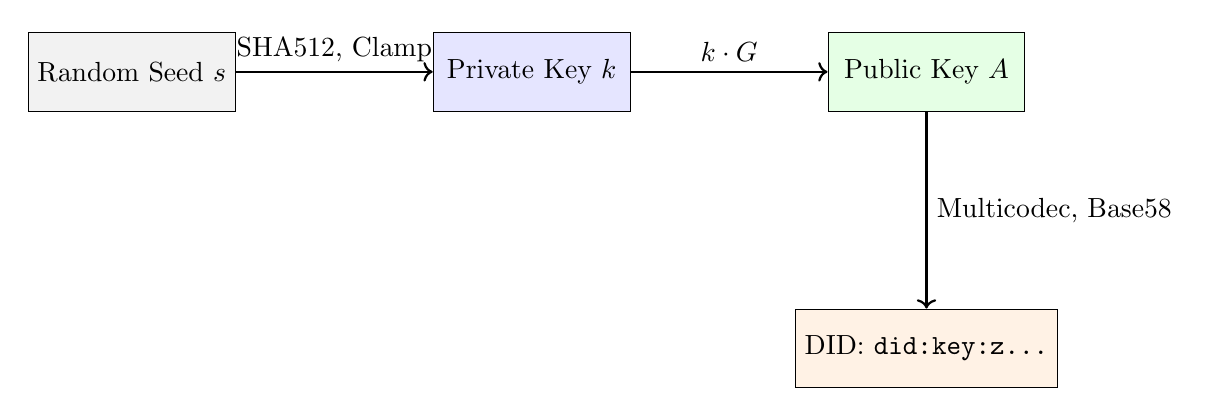
\begin{tikzpicture}[node distance=2.5cm, auto]
    \node[draw, rectangle, fill=gray!10, minimum width=2.5cm, minimum height=1cm] (seed) {Random Seed $s$};
    \node[draw, rectangle, fill=blue!10, right=of seed, minimum width=2.5cm, minimum height=1cm] (priv) {Private Key $k$};
    \node[draw, rectangle, fill=green!10, right=of priv, minimum width=2.5cm, minimum height=1cm] (pub) {Public Key $A$};
    \node[draw, rectangle, fill=orange!10, below=of pub, minimum width=3cm, minimum height=1cm] (did) {DID: \texttt{did:key:z...}};
    \draw[->, thick] (seed) -- node[above] {SHA512, Clamp} (priv);
    \draw[->, thick] (priv) -- node[above] {$k \cdot G$} (pub);
    \draw[->, thick] (pub) -- node[right] {Multicodec, Base58} (did);
  \end{tikzpicture}
  \caption{Ed25519 Key Generation and DID Encoding}
\end{figure}

\paragraph{Security and Decentralization}
This process ensures:
\begin{itemize}
  \item No central authority is required for identity issuance.
  \item Private keys never leave the user's device.
  \item All identity proofs and signatures are verifiable by any node.
\end{itemize}

\subsection{Commitment Hashes}
To register on the blockchain, a user publishes a cryptographic commitment. This is a hash (typically SHA-256) of their public key and selected metadata, canonicalized to ensure deterministic results. The commitment:
\begin{itemize}
  \item Proves the user's eligibility without revealing sensitive information.
  \item Is unique and non-replayable, enforced by blockchain consensus.
  \item Serves as the leaf in the Merkle accumulator.
\end{itemize}

\subsection{Merkle Accumulator}
All commitments are stored in an append-only log. Periodically, the blockchain computes a Merkle root over these commitments:
\begin{itemize}
  \item Each commitment is a leaf in the Merkle tree.
  \item The Merkle root summarizes the current set of eligible identities.
  \item Users can generate a Merkle proof (path of sibling hashes) to prove membership without revealing their identity.
\end{itemize}

\subsection{Zero-Knowledge Proofs (ZKP)}
For privacy-preserving voting, the system uses zero-knowledge proofs (ZKP), specifically SNARKs (Succinct Non-interactive Arguments of Knowledge):
\begin{itemize}
  \item The wallet generates a proof that it knows a valid commitment included in the Merkle root.
  \item The proof also demonstrates knowledge of a secret used to compute a \textbf{nullifier}, which is unique per vote context.
  \item The nullifier prevents double voting (one-person-one-vote) without linking votes to identities.
  \item The blockchain verifies the proof and nullifier uniqueness, ensuring both eligibility and anonymity.
\end{itemize}

\subsection{Poseidon Hash Function}
Poseidon is a cryptographic hash function optimized for use in SNARK circuits:
\begin{itemize}
  \item Used for hashing within the ZKP circuits (e.g., Merkle tree, nullifier computation).
  \item Parameters (matrices, rounds, constants) are generated deterministically and must be identical for all nodes.
  \item Poseidon ensures efficient, secure hashing compatible with zero-knowledge proofs.
\end{itemize}

\subsection{Signature Verification}
All transactions and identity operations are signed using Ed25519:
\begin{itemize}
  \item The blockchain verifies signatures to ensure authenticity and integrity.
  \item Only the holder of the private key can produce valid signatures or proofs.
\end{itemize}

\subsection{Privacy and Security Guarantees}
\begin{itemize}
  \item \textbf{Anonymity:} ZKP and nullifiers ensure actions cannot be linked to identities.
  \item \textbf{Eligibility:} Only registered commitments can participate; Merkle proofs guarantee membership.
  \item \textbf{Integrity:} All data is signed and hashed; tampering is detectable.
  \item \textbf{Transparency:} All verification is decentralized; no trusted third party is required.
\end{itemize}

\bigskip
\begin{itemize}[noitemsep]
  \item \textbf{Server backend:} HTTP API, consensus and security modules, storage layer, and identity issuance/verification components.
  \item \textbf{Shared domain models:} Core types used across components (transactions, blocks, accounts, laws, votes, proposals).
  \item \textbf{Cryptography module:} Key generation, signature handling, hashing, and serialization utilities.
  \item \textbf{Web interface:} Single-page application frontend for user interaction and data presentation.
  \item \textbf{Command-line wallet:} CLI for key management, credential handling, and transaction submission.
  \item \textbf{Migrations:} Ordered SQL scripts used to evolve the database schema safely.
  \item \textbf{Tests:} Unit and integration tests used to validate correctness and migration safety.
\end{itemize}

\begin{figure}[h!]
  \centering
  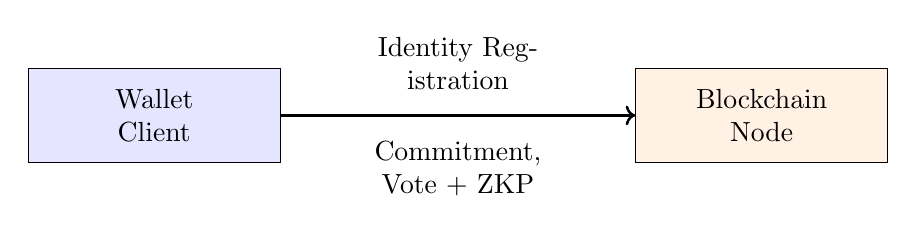
\begin{tikzpicture}[node distance=4.5cm, auto]
  \node[draw, rectangle, fill=blue!10, minimum width=3.2cm, minimum height=1.2cm, align=center] (wallet) {Wallet\\Client};
  \node[draw, rectangle, fill=orange!10, right=of wallet, minimum width=3.2cm, minimum height=1.2cm, align=center] (blockchain) {Blockchain\\Node};

  \draw[->, thick] (wallet) -- node[above, text width=3cm, align=center, yshift=0.2cm] {Identity Registration} (blockchain);
  \draw[->, thick] (wallet) -- node[below, text width=3cm, align=center, yshift=-0.2cm] {Commitment,\\Vote + ZKP} (blockchain);
  \end{tikzpicture}
  \caption{Architecture Overview with TikZ (no overlap)}
  \label{fig:tikz-architecture}
\end{figure}

\section{Identity, Commitments, and Privacy-Preserving Proofs}
The platform implements a privacy-preserving identity and voting system, ensuring that each citizen can participate only once per vote, while keeping their action anonymous.

\subsection{Identity Registration and Commitments}
Citizens generate a local Ed25519 keypair and derive a decentralized identifier (DID, e.g., \texttt{did:key}). The wallet registers its identity directly on the blockchain by publishing a canonicalized commitment (e.g., hash of public key and metadata). The blockchain validates uniqueness and eligibility according to its consensus rules. No central authority or government server is involved.

\subsection{Merkle Accumulator and Membership Proofs}

\paragraph{Formal Definition of Merkle Tree Construction}
Let $C_1, C_2, \ldots, C_n$ be the set of identity commitments. The Merkle tree is a binary tree where:
\begin{itemize}
  \item Each leaf node is $L_i = H(C_i)$, where $H$ is a cryptographic hash function (e.g., SHA-256 or Poseidon).
  \item Each internal node is $N_j = H(L_{j_1} \Vert L_{j_2})$, where $\Vert$ denotes concatenation.
  \item The Merkle root $R$ is the hash at the top of the tree, summarizing all commitments.
\end{itemize}

\begin{equation}
  L_i = H(C_i)
\end{equation}
\begin{equation}
  N_j = H(L_{j_1} \Vert L_{j_2})
\end{equation}
\begin{equation}
  R = \text{MerkleRoot}(C_1, \ldots, C_n)
\end{equation}

\paragraph{Membership Proof Generation}
To prove that a commitment $C_k$ is included in the Merkle root $R$, the user provides a membership proof (Merkle path):
\begin{itemize}
  \item The path consists of the sibling hashes $S_1, S_2, \ldots, S_d$ along the path from leaf $L_k$ to the root, where $d$ is the tree depth.
  \item At each level, the user reveals whether $L_k$ is a left or right child.
  \item The verifier recomputes the hashes up to the root and checks that the result matches $R$.
\end{itemize}

\begin{equation}
  ext{Given } L_k, S_1, \ldots, S_d,\quad R' = H\bigl(\ldots\, H\bigl(H(L_k\Vert S_1)\Vert S_2\bigr)\ldots\bigr)
\end{equation}
\begin{equation}
  ext{Accept if } R' = R.
\end{equation}


\paragraph{Schematic: Merkle Tree and Membership Proof}
\begin{figure}[h!]
  \centering
  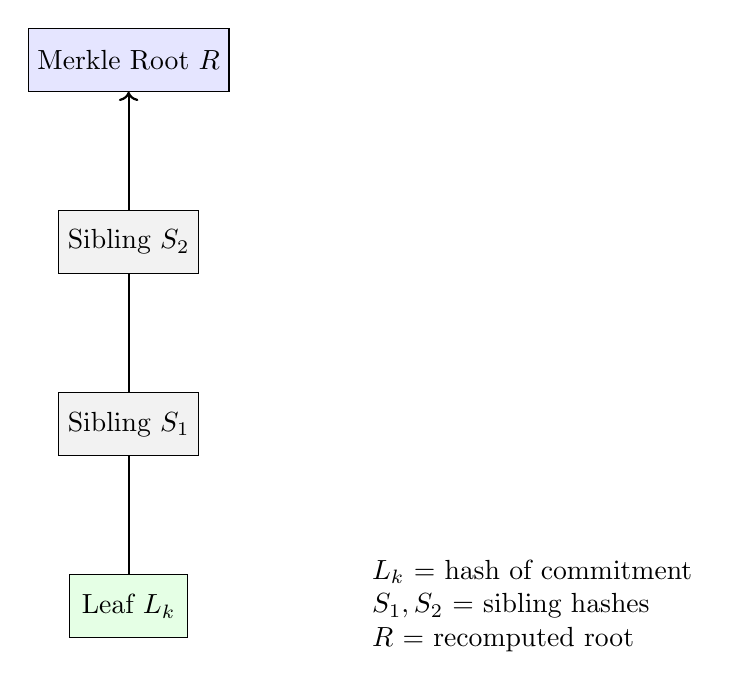
\begin{tikzpicture}[node distance=1.5cm, auto]
    \node[draw, rectangle, fill=green!10, minimum width=1.5cm, minimum height=0.8cm] (leaf) {Leaf $L_k$};
    \node[draw, rectangle, fill=gray!10, above=of leaf, minimum width=1.5cm, minimum height=0.8cm] (sib1) {Sibling $S_1$};
    \node[draw, rectangle, fill=gray!10, above=of sib1, minimum width=1.5cm, minimum height=0.8cm] (sib2) {Sibling $S_2$};
    \node[draw, rectangle, fill=blue!10, above=of sib2, minimum width=1.5cm, minimum height=0.8cm] (root) {Merkle Root $R$};
    \draw[->, thick] (leaf) -- (sib1) -- (sib2) -- (root);
    \node[right=2cm of leaf] (desc) {\begin{tabular}{l}
      $L_k$ = hash of commitment\\
      $S_1, S_2$ = sibling hashes\\
      $R$ = recomputed root\\
    \end{tabular}};
  \end{tikzpicture}
  \caption{Merkle Membership Proof: Path from Leaf to Root}
\end{figure}

\paragraph{Security Properties}
\begin{itemize}
  \item Membership proofs are succinct ($O(\log n)$ size) and do not reveal the position or value of other commitments.
  \item The Merkle root is collision-resistant if $H$ is secure.
  \item The proof does not reveal the user's identity or credential, only that their commitment is included.
\end{itemize}

\subsection{Zero-Knowledge Proofs (ZKP) for Anonymous Voting}

Zero-Knowledge Proofs (ZKP) are cryptographic protocols that allow a prover to convince a verifier that a statement is true, without revealing any information beyond the validity of the statement itself. In the context of anonymous voting, ZKPs are used to prove membership in a set (e.g., eligible voters) and to prevent double voting, all while preserving voter privacy.

	extbf{Formal Definition}

Let $\mathcal{S}$ be the set of eligible voters, represented as leaves in a Merkle tree. Each voter possesses a secret $s$ and a leaf value $l$. The Merkle root $r$ commits to the set $\mathcal{S}$.

The ZKP circuit proves the following statement:
\begin{align*}
  &\text{Given:} \\
  &\quad r = \text{MerkleRoot}(\mathcal{S}) \\
  &\quad l \in \mathcal{S} \\
  &\quad \text{Path}(l, r) \text{ is valid} \\
  &\quad \text{Nullifier} = \text{Poseidon}(\text{scope\_hash}, s) \\
  &\text{Prove:} \\
  &\quad l \text{ is a member of } \mathcal{S} \text{ and Nullifier is correctly computed}
\end{align*}

	extbf{Circuit Implementation}

The Rust implementation (\texttt{zkp.rs}) defines a circuit \texttt{MembershipNullifierCircuit} with the following public inputs:
\begin{itemize}
  \item Merkle root $r$
  \item Nullifier $n$
  \item Scope hash $h$
\end{itemize}
Private witnesses:
\begin{itemize}
  \item Leaf $l$
  \item Merkle path (siblings, directions)
  \item Secret $s$
\end{itemize}

The circuit enforces:
\begin{enumerate}
  \item The leaf $l$ and its Merkle path reconstruct the root $r$ using the Poseidon hash function.
  \item The nullifier $n$ is computed as $n = \text{Poseidon}(h, s)$, binding the vote to the scope and secret, preventing double voting.
\end{enumerate}

	extbf{Poseidon Hash:}
Poseidon is a SNARK-friendly hash function. The parameters are deterministically generated and injected as constants in the circuit:
\begin{align*}
  n &= \text{Poseidon}(h, s) \\
  r &= \text{MerkleRoot}(l, \text{path}; \text{Poseidon})
\end{align*}

	extbf{Proof Generation and Verification}

The proof is generated using the Groth16 SNARK protocol:
\begin{itemize}
  \item The circuit is instantiated with the voter's secret, leaf, and Merkle path.
  \item The proof is created with the proving key, and public inputs are exposed.
  \item Verification checks that the proof is valid for the given public inputs $(r, n, h)$.
\end{itemize}

	extbf{Code Reference:}
See \texttt{prove\_membership\_nullifier} in \texttt{zkp.rs} for the exact implementation:
\begin{itemize}
  \item Maps hex inputs to field elements.
  \item Loads Poseidon parameters.
  \item Synthesizes the circuit and checks satisfiability.
  \item Generates and verifies the Groth16 proof.
\end{itemize}

	extbf{Schematic Diagram}

\begin{center}
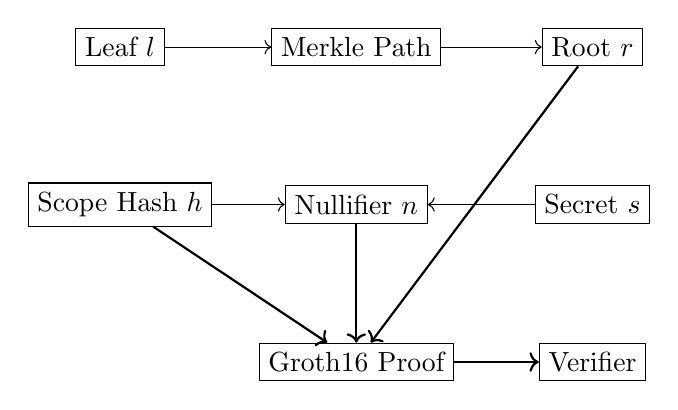
\begin{tikzpicture}[node distance=2.5cm and 2.5cm, auto]
  % Merkle tree (top row)
  \node (leaf) [draw, rectangle] at (0,0) {Leaf $l$};
  \node (path) [draw, rectangle] at (3,0) {Merkle Path};
  \node (root) [draw, rectangle] at (6,0) {Root $r$};
  \draw[->] (leaf) -- (path);
  \draw[->] (path) -- (root);

  % Nullifier (middle row)
  \node (scope) [draw, rectangle] at (0,-2) {Scope Hash $h$};
  \node (secret) [draw, rectangle] at (6,-2) {Secret $s$};
  \node (nullifier) [draw, rectangle] at (3,-2) {Nullifier $n$};
  \draw[->] (scope) -- (nullifier);
  \draw[->] (secret) -- (nullifier);

  % Proof (bottom row)
  \node (proof) [draw, rectangle] at (3,-4) {Groth16 Proof};
  \draw[->, thick] (root) -- (proof);
  \draw[->, thick] (nullifier) -- (proof);
  \draw[->, thick] (scope) -- (proof);

  % Verification (far right)
  \node (verify) [draw, rectangle] at (6,-4) {Verifier};
  \draw[->, thick] (proof) -- (verify);
\end{tikzpicture}
\end{center}

	extbf{Security and Privacy}
\begin{itemize}
  \item \textbf{Anonymity:} The proof reveals no information about the voter's identity or secret.
  \item \textbf{Unlinkability:} The nullifier prevents double voting without linking votes to identities.
  \item \textbf{Soundness:} Only eligible voters can produce valid proofs.
\end{itemize}

	extbf{Critical Review and TODOs}
\begin{itemize}
  \item Ensure Poseidon parameters are synchronized across all nodes (see \texttt{poseidon\_params\_hash}).
  \item Audit the circuit for edge cases (e.g., path length, input ordering).
  \item Extend the circuit for additional constraints (e.g., vote validity, time windows).
\end{itemize}

\subsection{Security and Privacy Properties}
\begin{itemize}
  \item Private keys never leave the wallet; all signatures and proofs are generated locally.
  \item The blockchain itself validates identity registration, eligibility, and uniqueness.
  \item No central authority is required; all verification is decentralized and transparent.
  \item All votes and actions are unlinkable to identities, thanks to ZKP and nullifiers.
\end{itemize}

\subsection{Example Identity Commitment}
\begin{lstlisting}[language=JSON,caption={Minimal Citizen Commitment}]
{
  "did": "did:key:zSUBJECT",
  "pubkey": "ed25519:...",
  "country": "FR",
  "over18": true,
  "roles": ["citizen"],
  "commitment_hash": "..."
}
\end{lstlisting}

\subsection{Sequence Diagram (Conceptual)}
\begin{verbatim}
Wallet -> Blockchain: Register identity (commitment)
Blockchain: Validate uniqueness, eligibility
Wallet -> Blockchain: Submit vote with ZKP and nullifier
Blockchain: Verify ZKP, check nullifier uniqueness, record vote
\end{verbatim}

\chapter{Components ("Blocks")}
\section{Common (Domain Model)}
The \texttt{common} crate defines core domain structures:
\begin{itemize}[noitemsep]
  \item \textbf{Transaction}: includes \texttt{id}, \texttt{transaction\_type}, \texttt{sender}, \texttt{timestamp}, \texttt{signature}, \texttt{nonce}, \texttt{fee}, and \texttt{data\_hash}. A \texttt{verify()} method checks integrity and signatures.
  \item \textbf{Blockchain, Block, Account, Law, Vote, Proposal}: types representing the ledger and governance entities.
  \item \textbf{Identity (feature-gated)}: DID utilities, canonical JSON and commitment hashing, VC helpers.
\end{itemize}

\section{Blockchain}

\subsection{API}
The API is built with http protocol. Routes cover general blockchain operations and identity endpoints. The server can be started normally or in migrate-only mode.

% No identity issuer: all identity registration and verification is performed by the blockchain consensus and smart contract logic.

\subsection{Security Module}
Security covers:
\begin{itemize}[noitemsep]
  \item Signature verification via \texttt{Transaction::verify()}.
  \item Proof-of-work simulation with configurable difficulty.
  \item Double-spend detection hardened with per-sender nonces: transactions must use strictly increasing nonces compared to chain history; duplicates within a block are rejected. A fallback heuristic (same sender and \texttt{data\_hash}) protects older clients.
\end{itemize}

\section{Wallet CLI}
The CLI provides a scaffold for interactions (to be expanded). Future work includes commands for submitting transactions, querying the chain, and handling identity credentials.

\chapter{Data Model and Schema}
\section{Core Tables}
At minimum, the schema includes:
\begin{itemize}[noitemsep]
  \item \textbf{blocks}, \textbf{transactions}, \textbf{accounts}, \textbf{laws}, \textbf{votes}
  \item \textbf{identity\_commitments}: stores canonicalized commitment hashes and signed artifacts; unique \texttt{commitment\_hash} ensures idempotence.
  \item \textbf{schema\_migrations}: migration bookkeeping.
\end{itemize}

\section{Identity Commitments}
Commitment hashes are computed over canonicalized unsigned credential JSON (stable ordering). The storage layer inserts commitments idempotently via a uniqueness constraint.

\chapter{APIs}
\section{Identity}
\begin{itemize}[noitemsep]
  \item \textbf{POST /issuer/issue}: Issues a verifiable credential for a subject DID; returns the signed credential and signing artifacts.
  \item \textbf{POST /issuer/verify}: Verifies a provided credential by canonicalization, digest check, key recovery (did:key), signature verification, and method coherence.
\end{itemize}
\noindent Other blockchain-related routes exist for accounts, laws, votes, and P2P operations (see server sources).

\chapter{Security Considerations}
\section{Threats and Controls}
\begin{itemize}[noitemsep]
  \item \textbf{Double spend:} prevented via per-sender nonces and intra-block duplication checks; heuristic fallback for legacy clients.
  \item \textbf{Replay:} nonces and \texttt{data\_hash} uniqueness reduce replay viability.
  \item \textbf{Integrity:} deterministic canonicalization and digesting; Ed25519 signatures.
  \item \textbf{PoW abuse:} difficulty parameter validated during block mining.
\end{itemize}

\chapter{Build, Run, and Tooling}
Workspace tasks provide repeatable commands (build, test, run services). The server supports \texttt{--migrate} to apply DB migrations without starting network services. The web interface uses Trunk for development and hot reload.

\chapter{Testing}
Unit tests cover cryptographic primitives, identity hashing, and server-side security behaviors. Integration tests assert migration correctness and storage idempotence. The full test suite passes at the time of writing (warnings remain to be cleaned up).

\chapter{Future Work}
\begin{itemize}[noitemsep]
  \item Persist and reload issuer keypairs securely to stabilize DID across restarts.
  \item Expand negative-path identity tests (tampering, expiry, verification method mismatches).
  \item Replace heuristic double-spend fallback with explicit inputs (UTXO) or stricter account-state checks.
  \item Add diagrams (architecture, sequence charts) and a thorough API reference.
  \item Performance benchmarks and capacity planning (block times, throughput).
  \item Deployment guidelines (containerization, CI/CD) and operational runbooks.
\end{itemize}

\appendix
\chapter{Repository Layout (Excerpt)}
\begin{verbatim}
blockchain-server/
  src/ (API, issuer, security, storage, consensus, network)
common/ (domain models; optional identity feature)
crypto-lib/ (keys, signatures, hashing)
web-interface/ (Yew + Trunk)
wallet-cli/
migrations/ (0000_init.sql, 0001_identity_commitments.sql)
tests/ (integration tests)
\end{verbatim}

% \bibliographystyle{plain}
% \bibliography{references}

\end{document}
% =====================
\chapter*{Critical TODOs and Review}
\addcontentsline{toc}{chapter}{Critical TODOs and Review}

This section lists explicit, critical TODOs and review points for improving the rigor, completeness, and clarity of this university report. Each item is explained in detail, with suggestions for how to address it.

\section*{Architecture and Conceptual Clarity}
\begin{itemize}
  \item \textbf{Logical Architecture Diagram:} The current diagram is minimal. Add a comprehensive diagram showing all logical components, their interactions, and data flows (not just wallet/blockchain). Use clear labels and explain each arrow and block.
  \item \textbf{Component Responsibilities:} For each major block (wallet, blockchain node, web interface, etc.), provide a detailed description of its responsibilities, boundaries, and how it interacts with other components. Avoid implementation details, focus on conceptual roles.
  \item \textbf{Data Flow and Trust Boundaries:} Explicitly describe how data moves between components, where trust boundaries exist, and how privacy is preserved at each step.
\end{itemize}

\section*{Cryptographic Mechanisms}
\begin{itemize}
  \item \textbf{Formal Definitions:} For each cryptographic primitive (Ed25519, SHA-256, Poseidon, Merkle, SNARK), provide a formal definition, security assumptions, and why it was chosen for this context.
  \item \textbf{Threat Model:} Critically analyze the threat model. What attacks are possible? What are the limitations of the current cryptographic choices? Are there privacy or integrity risks not addressed?
  \item \textbf{Parameter Distribution:} The report mentions Poseidon parameters must be identical on all nodes, but does not specify how this is enforced or distributed. Add a section on parameter management and risks of inconsistency.
\end{itemize}

\section*{Identity and Privacy}
\begin{itemize}
  \item \textbf{Anonymity Guarantees:} The report claims anonymity via ZKP and nullifiers, but does not formally define anonymity or linkability. Add a subsection on privacy guarantees, with references to formal definitions (e.g., unlinkability, non-traceability).
  \item \textbf{Eligibility and Revocation:} How is eligibility managed over time? Can identities be revoked or updated? What happens if a user loses their key?
  \item \textbf{Commitment Uniqueness:} The process for ensuring commitment uniqueness is described, but edge cases (collisions, replay, Sybil attacks) are not discussed. Add a critical analysis.
\end{itemize}

\section*{APIs and Data Model}
\begin{itemize}
  \item \textbf{API Reference:} The API section is brief. Add a full reference for each endpoint, including request/response schemas, error handling, and security considerations.
  \item \textbf{Schema Excerpts:} Include explicit schema definitions for core tables (blocks, transactions, accounts, votes, identity	extunderscore commitments), with explanations of constraints and relationships.
  \item \textbf{Migration Details:} The migration process is mentioned, but not described in detail. Add a section on migration loader, file naming conventions, transactional semantics, and failure recovery.
\end{itemize}

\section*{Security and Threats}
\begin{itemize}
  \item \textbf{Replay and Double Spend:} The report mentions nonce and data	extunderscore hash uniqueness, but does not provide a formal security proof or discuss edge cases. Add a rigorous analysis.
  \item \textbf{Consensus Assumptions:} What are the assumptions about the blockchain consensus? Is it PoW, PoS, or something else? What are the risks and limitations?
  \item \textbf{Operational Security:} Add guidelines for key rotation, backup, and recovery. Discuss risks of key compromise and mitigation strategies.
\end{itemize}

\section*{Testing and Evaluation}
\begin{itemize}
  \item \textbf{Test Coverage:} The report claims unit and integration tests exist, but does not provide coverage metrics or examples. Add a section on test methodology, coverage, and critical test cases.
  \item \textbf{Performance Benchmarks:} No performance data is provided. Add benchmarks for block times, transaction throughput, and ZKP generation/verification times.
  \item \textbf{Limitations and Future Work:} Critically discuss what is missing, what is out of scope, and what should be addressed in future versions.
\end{itemize}

\section*{General Academic Rigor}
\begin{itemize}
  \item \textbf{References and Citations:} The report lacks citations to standards (DID, VC, Ed25519, SNARKs, Poseidon, etc.). Add a bibliography and cite relevant literature.
  \item \textbf{Glossary:} Add a glossary of technical terms for clarity.
  \item \textbf{Critical Review:} For each section, add a paragraph critically assessing what is well-covered and what is missing or unclear.
\end{itemize}

\bigskip
